\section{Member 5: calibration and the prior-shift correction}
\label{sec:m5}
\textbf{Code:} \code{calibration.py}, \code{prior\_shift.py}, and in \code{experiments/}:
\code{task3\_calibration.py}, \code{t5\_prior\_correction.py}.

\paragraph{Measuring probabilities.}
Accuracy only asks whether $\post$ is on the right side of $0.5$. Our rule compares $\post$ with
$0.3$ and $0.97$, so it needs $\post$ to be \emph{calibrated}: of the emails given $\post=0.8$, about
$80\%$ should be spam. \code{calibration.py} implements the log-loss, the Brier score, the expected
calibration error (ECE: the average gap between forecast and observed spam rate over 10 bins),
reliability diagrams, temperature scaling, $\post_T=\sigm(\logit\post/T)$, which makes a model more
($T<1$) or less ($T>1$) confident, and Platt scaling, $\post'=\sigm(A\logit\post+B)$, which re-calibrates a
model on validation data. The tests check
every score against hand-worked examples and scikit-learn.

\begin{table}[!htbp]
\centering\footnotesize\setlength{\tabcolsep}{3.5pt}
\input{\resultsdir/c4_scores.tex}
\caption{Forecast quality on test data (mean $\pm$ standard error, 20 splits). Accuracy uses the cut
$0.5$; Cost and Inspected are for the rule with inspection ($\cfp=10$, $\cfn=1$, $\ci=0.3$). Spambase
uses $\log(1+x)$ features. ``+ Platt'': re-calibrated on validation data.}
\label{tab:c4}
\end{table}

\paragraph{Results.}
On synthetic data, where both models' assumptions hold, they are as good as the true posterior
(Table~\ref{tab:c4}), which checks the code. On Spambase, logistic regression beats the Gaussian
model on every score (log-loss $0.185$ against $0.224$, ECE $0.021$ against $0.039$) and costs
$0.124$ per email against $0.142$, although their accuracies differ by only $1.3$ points. The
reliability diagram (Figure~\ref{fig:c4-rel}) shows where: the Gaussian model underestimates spam for
$\post$ between $0.3$ and $0.6$, exactly where the lower threshold sits.

\begin{figure}[!htbp]
\centering
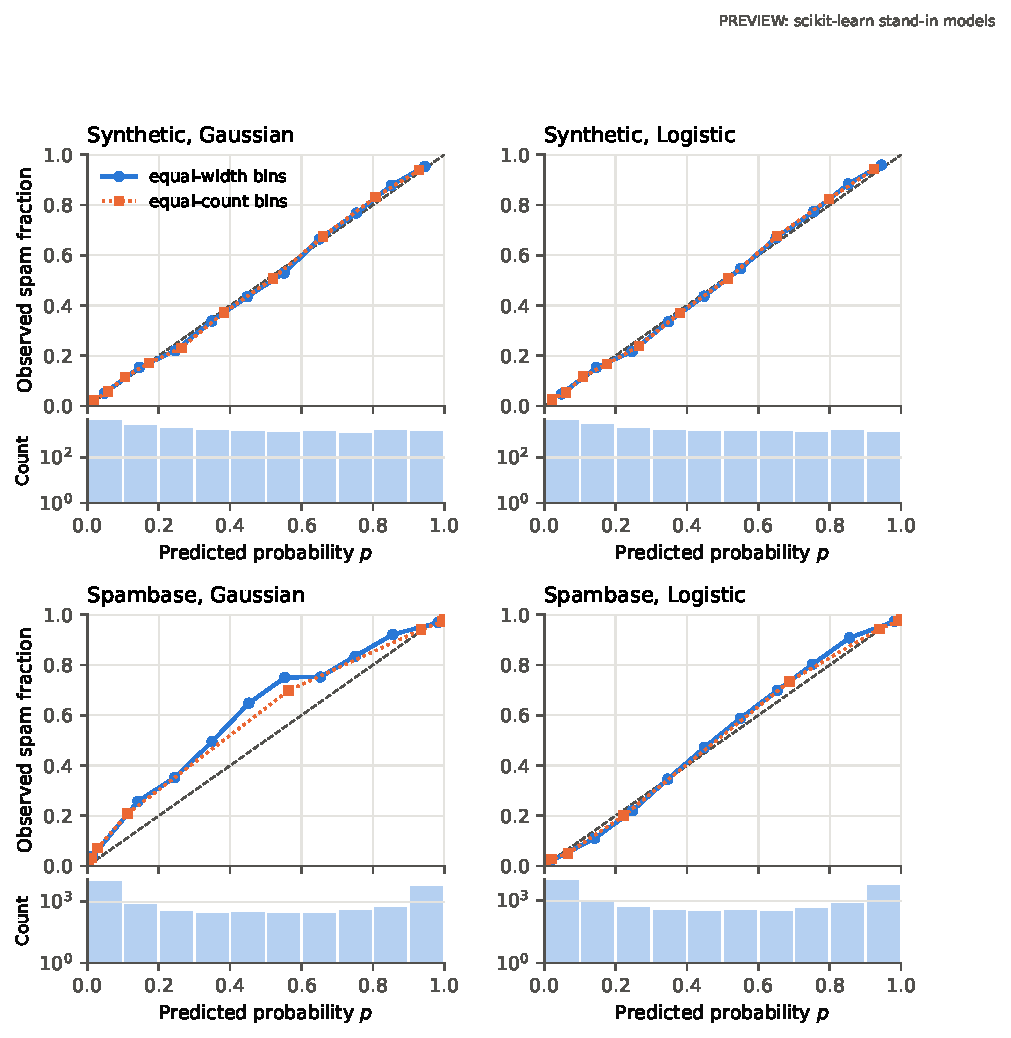
\includegraphics[width=0.62\linewidth]{c4_reliability.pdf}
\caption{Reliability diagrams on the test parts of all 20 splits. Points above the diagonal mean the
model underestimates spam; the histograms count the forecasts in each bin (log scale).}
\label{fig:c4-rel}
\end{figure} Platt scaling repairs much of this: its ECE falls to $0.024$ and its cost to $0.132$.

\paragraph{Same accuracy, different cost.}
Temperature scaling never moves a probability across $0.5$, so it leaves accuracy unchanged, but it
changes which emails pass $0.3$ and $0.97$ (Table~\ref{tab:c4-temp}). Making the logistic model
over-confident ($T=0.4$) raises the number of real emails sent to spam from $3.8$ to $10.5$ per test
split and the cost by a third, at the same $93.6\%$ accuracy. Log-loss detects this; the Brier score
barely moves.

\begin{table}[!htbp]
\centering\footnotesize\setlength{\tabcolsep}{4pt}
\input{\resultsdir/c4_temperature.tex}
\caption{Logistic regression on Spambase after temperature scaling (mean $\pm$ standard error).}
\label{tab:c4-temp}
\end{table}

\paragraph{Correcting for a new spam rate.}
A filter trained where $39\%$ of emails are spam may be used where only $5\%$ are. If spam still
looks the same and only the proportion $\pio$ changes to $\pion$, every email's log-odds should move
by the same amount, so \code{prior\_shift.py} corrects the model's output as
\[
  \post'=\sigm\!\big(\logit\post+\lshift\big),\qquad
  \lshift=\log\frac{\pion}{1-\pion}-\log\frac{\pio}{1-\pio}.
\]
For example, a model trained at $\pio=0.5$ and deployed at $\pion=0.1$ turns $\post=0.98$ into
$\post'\approx0.845$, so that email is inspected instead of filed as spam. Equivalently, the
thresholds can be moved instead of the probabilities. \code{t5\_prior\_correction.py} plots both views
(Figure~\ref{fig:t5}). Member 1 tests the correction in the next section.

\begin{figure}[!htbp]
\centering
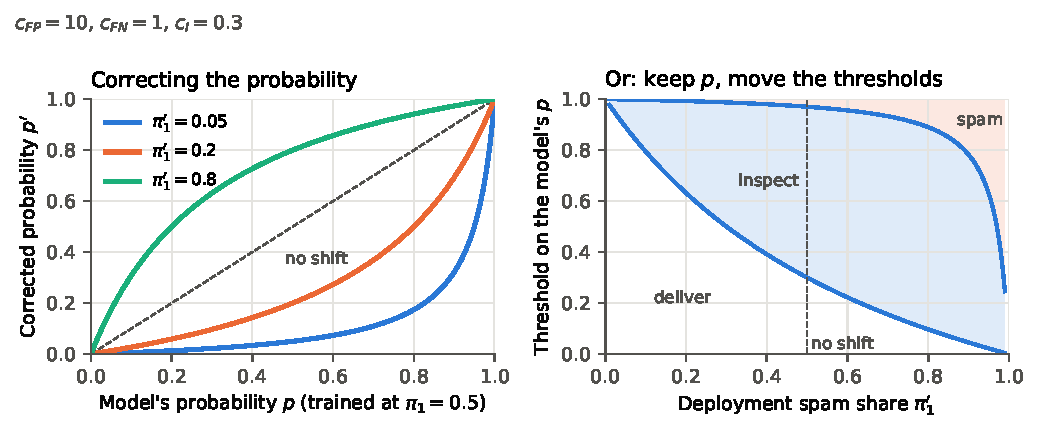
\includegraphics[width=0.92\linewidth]{t5_prior_correction.pdf}
\caption{Prior-shift correction for a model trained at $\pio=0.5$. Left: corrected $\post'$ against
$\post$. Right: the equivalent thresholds on the uncorrected $\post$ for every deployment rate $\pion$;
the shaded band is the inspect region.}
\label{fig:t5}
\end{figure}
